% !TEX root = /home/frank/School/thesis_text/thesis.tex
% $Id: $


\documentclass[a4paper,12pt]{report}

% The following makes latex use nicer postscript fonts.
\usepackage{times}
\usepackage[dutch,english]{babel}
%\usepackage[colorlinks,urlcolor=blue,linkcolor=blue]{hyperref}


 
%%%%%%%%%%%%%%%%%%%%%
%					%
%	VUB Title Page	%
%					%
%%%%%%%%%%%%%%%%%%%%%

\usepackage{vubtitlepage}

\author{			Frank Vanbever}
\title{			Performance Analysis of a Real-Time Video Processing System}

\promotortitle{	Promotors}
\promotor{		Dr. ir. Erik D'Hollander\\
				Dr. An Braeken}

\advisortitle{	Advisors}					
\advisors{		Ing. Bruno Tiago Da Silva Gomes}

\faculty{		Faculty of Applied Sciences and Engineering}

\department{		INDI Department}
\reason{			Graduation thesis submitted in partial fulfillment of the requirements
				for\\ the degree of Master of Science in Applied Engineering: Electronics-ICT}
\date{			January 2014}







%%%%%%%%%%%%%%%%%%%%%%%%%%%%%%%%%
%								%
%	Personal Package Includes	%
%								%
%%%%%%%%%%%%%%%%%%%%%%%%%%%%%%%%%


\usepackage{graphicx}
\usepackage{listings}
\usepackage[usenames,dvipsnames]{xcolor}
\usepackage{lscape}
\usepackage{amsmath}
\usepackage{tabularx}
\usepackage{multicol}
\usepackage{float}
\usepackage{booktabs}
\usepackage{afterpage}
\usepackage[toc,acronym]{glossaries}

%%%%%%%%%%%%%%%%%%%%%%%%%
%						%
%	Personal Settings	%
%						%
%%%%%%%%%%%%%%%%%%%%%%%%%

% set the lenght of the indentation of a new paragraph to 0
\setlength{\parindent}{0pt}

% set some parameters for the listing.
\lstset{language=C,
		belowskip=1em,
		aboveskip=1em,
		basicstyle=\scriptsize,
		keywordstyle=\color{blue},
        stringstyle=\color{red},
        commentstyle=\color{NavyBlue},
        morecomment=[l][\color{magenta}]{\#}
        }


%%%%%%%%%%%%%%%%%%%%%%%%%
%						%
%	Personal Commands	%
%						%
%%%%%%%%%%%%%%%%%%%%%%%%%


\newcommand{\skipbig}[1]{\bigskip #1 \bigskip}
\newcommand{\hlsdirective}[1]{\begin{small} \texttt{#1} \end{small}}

\newcommand{\quotationmarks}[1]{ ``#1''}

\newcommand{\abbreventry}[2]{\textbf{#1}: #2\\}

\newcommand{\emptypage}[0]{\newpage \mbox{}}


\makeglossaries


%%%%%%%%%%%%%%%%%%%%%%%%%%%%%
%							%
%	DOCUMENT BEGINS HERE	%
%							%
%%%%%%%%%%%%%%%%%%%%%%%%%%%%%

\begin{document}

\pagenumbering{gobble}
\maketitlepage

\emptypage
\emptypage
\emptypage

\maketitlepage
\emptypage

\pagenumbering{arabic}


% !TEX root = /home/frank/School/thesis_text/thesis.tex


\chapter*{Abstract}

There are many applications that could benefit form increased computing performance. In the past this need was mostly satisfied by Moore's law, which enabled hardware designers and programmers to continue supporting a sequential programming paradigm. However due to power constraints it proved unmaintainable to continue increasing the frequency. The need for processing power however kept rising, and Moore's law is still valid, so parallelism was introduced to enable an increase in performance. The CPU's used in desktop and server computers have become multi-core processors, and alternatives such as General Purpose Graphics Processing Units and Field Programmable Gate Arrays can offer extreme parallelism for applications that can benefit from it. The goal of this thesis is to study a new type of heterogeneous architecture, the Zynq SoC form Xilinx. This chip is a combination of a dual core ARM processor and an FPGA on the same die. Ideally this brings the best features of both processors to the table: the ease of use and floating point performance of the CPU and the massively parallel performance of the FPGA. In the first chapter an introduction is given to the current state of parallel computing. A summary is given of the different types of computing components is given, as well as an introduction to a system for determining which processing unit is most fit to run a certain algorithm. The second chapter gives an overview of the features of the Zynq platform, discussing both the processing system, the programmable logic and the interconnection between these two. The toolchain used to develop for this platform is introduced, as well as the video processing system used to perform the performance analysis. This system, the Zynq Base Targeted Reference Design is a real-time video processing system which has stringent throughput requirements. The complete stack is discussed: the hardware implementation, the operating system and the user application. In the third chapter details High Level Synthesis, a technique for converting high level programming languages into hardware. The many features of the tool used for this thesis, Vivado HLS, are also discussed in this chapter. In the fourth chapter the factors influencing the performance are discussed, as well as the roofline model, a way to visually represent the performance of a system. Concepts form this roofline model are used to interpret the performance of the system.
% !TEX root = /home/frank/School/thesis_text/thesis.tex

\chapter*{Abstract (NL)}

\begin{otherlanguage}{dutch}


Er zijn vele toepassingen die baat hebben die baat hebben bij een toegenomen prestatie van de computer die ze uitvoert. In het verleden zorgde de wet van Moore ervoor dat ontwerpers en programmeurs het sequenti\"ele paradigma konden blijven toepassen. Door limieten in de fysica van halfgeleiders werd het halverwege het vorige decennium onhoudbaar om dit model nog te volgen. De nood aan extra performantie bleef echter bestaan, en Moore's law was nog steeds geldig. Omwille van deze redenen werd parallellisme geïntroduceerd om voor bepaalde parallelle toepassingen te gaan versnellen. Vandaag hebben processoren in desktops en servers een multi-core processor aan boord, en alternatieven zoals de GPGPU of de FPGA kunnen extreem parallellisme bieden voor applicaties die hier baat van kunnen hebben.Het doel van deze thesis is om de performantie van een nieuw type heterogene architectuur te bestuderen, de Zynq SoC van Xilinx. Deze chip combineert een dual core ARM processor en een FPGA op dezelfde chip. Idealiter zou deze de voordelen van deze beide moeten samenbrengen in 1 verpakking: het gebruiksgemak en performantie bij floating-point berekeningen van de CPU en het doorgedreven parallellisme van de FPGA.
In het eerste hoofdstuk wordt een introductie gegeven tot de huidige toestand van parallel processing. De meest courante parallelle processors worden beschreven evenals een systeem voor het classificeren van parallelle algoritmes. Het tweede hoofdstuk begint met een beschrijving van het Zynq platform, waarbij de processor, de FPGA en de verbindingen tussen deze 2 besproken worden. Het FPGA ontwerp voor videobewerking dat gebruikt wordt voor deze thesis, de Zynq Targeted Reference Design is een real-time videobewerkingssysteem met strenge vereisten voor de doorvoer van het systeem. De volledige stack wordt besproken, gaande van de hardware over het besturingssysteem tot de eigenlijke applicatie. In het derde hoofdstuk wordt uitgelegd wat hoogniveausynthese is, een techniek om een hoogniveau programmeertaal om te zetten naar hardware. De eigenschappen van Vivado HLS, de gebruikte software, worden ook in dit hoofdstuk besproken. In het vierde hoofdstuk worden de factoren die de performantie van het systeem be\"invloeden besproken, evenals een systeem om de performantie visueel weer te geven:  het roofline model. Concepten van dit roofline model worden gebruikt om de performantie te interpreteren. 

\end{otherlanguage}
% !TEX root = /home/frank/School/thesis_text/thesis.tex


\chapter*{Preface}


I chose the topic of high performance computing because FPGA's are an interest of mine and it seemed challenging. Little did I know that I would be given the opportunity to study the Zynq platform, real cutting edge technology. To do this I had to acquire a lot of skills I did not previously have, and I improved a lot I did have. I learned a lot about hardware design using both VHDL and HLS tools, as well as embedded development, both for bare metal ARM and embedded Linux. The skills I have gained in creating this work will undoubtedly prove of great value in my future career as an engineer, in which I hope I can continue working on exciting systems such as the Zynq. \\

First of all I would like to thank my promotors, Dr. ir. Erik D'Hollander and Dr. An Braeken for their patience and support in guiding my work.\\

I would like to express my sincere gratitude to Bruno Da Silva for going above and beyond in helping me get to the bottom of the Zynq platform and inspiring me too keep pushing further. \\

Many thanks go out to Ing. Laurent Segers, Ing. Yannick Verbelen, Ing. Serge Kubera and everyone else at the Rapptorlab for putting up with me all this time and making me feel welcome.\\

Finally I would also like to thank my partner Stefanie Kneuts and Thomas Wyseur for taking the time to proof read this text. 





\emptypage

% Obligatory lists
\tableofcontents
\listoffigures
\listoftables
% !TEX root = /home/frank/School/thesis_text/thesis.tex


\chapter*{List of Abbreviations}
\begin{multicols}{2}
\abbreventry{CPU}{Central Processing Unit}
\abbreventry{FPGA}{Field Programmable Gate Array}
\abbreventry{GPGPU}{General Purpose Graphics Processing Unit}
\abbreventry{SoC}{System on Chip}
\abbreventry{TRD}{Targeted Reference Design}
\abbreventry{HLS}{High Level Synthesis}
\abbreventry{MOSFET}{Metal Oxide Semiconductor Field Effect Transistor}
\abbreventry{FLOPS}{Floating Point Operations}
\abbreventry{SIMD}{Single Instruction Multiple Data}
\abbreventry{LUT}{Look Up Table}
\abbreventry{DSP}{Digital Signal Processing}
\abbreventry{HDL}{Hardware Description Language}
\abbreventry{PS}{Processing System}
\abbreventry{PL}{Programmable Logic}
\abbreventry{APU}{Application Processor Unit}
\abbreventry{DDR}{Double Data Rate}
\abbreventry{IO}{Input/Output}
\abbreventry{AMBA}{Advanced Microcontroller Bus Architecture}
\abbreventry{AXI}{Advanced eXtensible Interface}
\abbreventry{HP}{High Performance}
\abbreventry{GP}{General Purpose}
\abbreventry{ACP}{accelerator Coherency Port}
\abbreventry{SCU}{Snoop Control Unit}
\abbreventry{OCM}{On Chip Memory}
\abbreventry{XPS}{Xilinx Platform Studio}
\abbreventry{SDK}{Software Development Kit}
\abbreventry{VDMA}{Video Direct Memory Access}
\abbreventry{HDMI}{High-Definition Multimedia Interface}
\abbreventry{UIO}{Userspace Input/Output}
\abbreventry{GUI}{Graphical User Interface}
\abbreventry{CP}{Computational performance}
\abbreventry{BW}{Bandwidth}
\abbreventry{CI}{Computational Intensity}
\abbreventry{SC}{Scalability}
\end{multicols}


\emptypage

% !TEX root = /home/frank/School/thesis_text/thesis.tex




\chapter{Introduction} 
Up until halfway the first decade of the new millennium it was possible to gain computing performance whilst also being able to maintain the sequential programming paradigm. This was due to Moore's law, stating that the number of transistors on integrated circuits double approximately every two years. There was no need for research into explicit parallelism because the next generation of computing devices was just around the corner. This new generation would increase the performance with zero effort required from the programmer.To perpetuate the sequential programming paradigm several innovations such as multiple issue, deep pipelines and out of order execution were introduced. These optimizations  were inefficient in both the use of transistors and power. Eventually it became impossible to progress any further whilst still supporting the sequential paradigm. The integrated circuit industry was unable to continue decreasing the size of MOSFETs whilst continuing to increase the clock frequency. The industry had hit what is called the power wall.
The solution to this problem was to turn to parallel processors, meaning that there is more than one processing unit working at a time. A lot of real world applications are parallel, and hardware can be made parallel with relative ease. The problem lies in the programming model, how to exploit this parallelism and make programming for these parallel architectures easier and transparent for the programmer.



\section{Computing Components}

\subsection{Multicore Processor}
The multicore processor is the solution presented for the aforementioned problems by the traditional CPU manufacturers such as Intel and AMD. The idea behind this type of processor is to place a number of cores (currently up to eight) on the same die. This presents a compromise between maintaining sequential performance whilst also providing a certain advantage of parallel processing. Parallel programming for these processors presents certain challenges, whilst their modest parallelism cannot provide a dramatic improvement in power performance. Multicore processors are unlikely to be a one-size-fits-all solution to the parallel problem.\cite{asanovic_landscape_????}

\subsection{Graphics Processing Units} 
Graphics processing units are a type of coprocessor used in traditional computers to process images for output to the display. However recently there has been an increased interest in the GPGPU, a general purpose graphics processing unit. These processors implement a different paradigm, namely the manycore paradigm. A  GPU is a processor with hundreds single instruction multiple data cores, each of which is heavily multi-threaded. Because of this large amount of cores the FLOPS (floating point operations per second) is unrivaled\cite{kirk_programming_2010}. GPU's, due to their SIMD (single instruction multiple data) nature present some problems, conditional execution paths for example, present a serious overhead on the GPU. GPU's are programmed with either OpenCL (open standard) or CUDA (proprietary to Nvidia)

\subsection{Field Programmable Gate Array} 
FPGAs are devices containing a vast amount of configurable logic linked by programmable connections. This logic is comprised of lookup tables (LUTs) grouped together into configurable logic blocks. Any combinatorial function can be programmed into these LUT's. Next to these uncommitted logic blocks a typical FPGA also contains several blocks with a specific function such as block ram and DSP multipliers. FPGAs are an interesting competitor in the parallel processing field because they are not constrained by the Von Neuman architecture. FPGAs follow the dataflow paradigm in which the data \emph{flows} through the logic. Implementing a data-flow is inherently parallel. The different stages in the datapath can also be made effectively sequential making the datapath a pipeline. The fine grained nature of FPGAs also means that the bitwidth can be adapted to the application.


\section{Berkeley dwarfs }

Image processing algorithms are very compute intensive. These makes them prime targets for exploiting parallelism and implementing them on parallel architectures. Which platform is the best fit is dependent on both the algorithm and the data. A common method to subdivide parallel algorithms is presented in , the so called \emph{dwarfs}. These 13 dwarfs are classes of algorithms in which the membership is defined by a similarity in computation and data movement.These 13 dwarfs are classes of algorithms in which the membership is defined by a similarity in computation and data movement.
The dwarfs are:

\begin{multicols}{2}
\begin{enumerate}
\item Dense Linear Algebra
\item Sparse Linear Algebra
\item Spectral Methods
\item N-Body Methods
\item Structured Grids
\item Unstructured Grids
\item MapReduce
\item Combinational Logic
\item Graph Traversal
\item Dynamic Programming
\item Backtrack and Branch-and-Bound
\item Graphical Models
\item Finite State Machines
\end{enumerate}
\end{multicols}

A thorough review of these dwarfs and what kind of computation and communication they entail goes beyond the scope of this document. An updated view can be found in \cite{asanovic_view_2009}.\
Finding out which platform is most suited for a dwarf is a labor intensive task. In \cite{inta_chimera:_2012} a theoretical analysis of dwarf performance on different accelerators in heterogeneous systems is given. A first point of note is that GPGPU's are unsurpassed in floating point arithmetic. Fixed point numbers are a way to overcome this problem. Another point to note is that conditional elements and  costly communication can wreak havoc on the accelerator's performance. In Figure \ref{img:venndiagram_chimera} the analysis is represented by a Venn diagram. In this diagram `*' denotes fixed point operations whilst `\^{}' denotes floating point operations.

\begin{figure}[H]
\centering
\includegraphics[scale=0.34]{/home/frank/School/thesis_text/images/venndiagram_chimera.png}
\caption{Analysis of different hardware accelerators in regards to performance on a certain dwarf \cite{inta_chimera:_2012} }
\label{img:venndiagram_chimera}
\end{figure}


\section{GUDI Project}

This thesis is inspired by the work of the GUDI project. GUDI is an acronym for \quotationmarks{A Combined \textbf{G}P-GP\textbf{U}/FPGA \textbf{D}esktop for accelerating \textbf{I}mage processing applications}. The research starts from the observation that there is a large need for computing power to process data using computationally intensive image processing algorithms. Conventional Off-the-shelf Desktop computers don't have the necessary processing power to satisfy this demand. A lot of image processing algorithms exhibit parallelism which can be exploited by the right architecture. Two such massively-parallel architectures are GP-GPU's and FPGA's. The GUDI project's goal is to investigate the possibilities and limitations of a computer with such a heterogeneous architecture. It is an investigation into the technologies and development tools and their performance in different situations. The means through which this is done is through the implementation and performance measurement of algorithms. The ultimate goal is to split an algorithm into several parts, executed on the technology (CPU,GPU,FPGA) most fit for the job so as to ensure optimal speed-ups.







% !TEX root = /home/frank/School/thesis_text/thesis.tex



\chapter{Platform Overview}

\section{Zynq-7000}


The Zynq-7000 System on Chip combines a dual core ARM Cortex-A9 with Xilinx programmable logic in a single device. This combination of a CPU and an FPGA on the same device is not a new phenomenon, with examples of previous generations being the PowerPC based Xilinx Virtex-II Pro and some models of the Virtex 4 and Virtex 5 series FPGA's. The main difference between the current generation and previous generations is the programming model used for these types of components. Whereas the focus in previous generations was on HDL design, nowadays the focus is more on programming with high level languages. (http://www.edn.com/electronics-products/other/4369562/Dual-ARM-Cortex-A9-MPCore-features-28-nm-low-power-programmable-logic-for-high-end-embedded-systems)
This device integrates a dual core ARM Cortex-A9 and Xilinx Programmable Logic in a single device. The communication between these two components goes through an ARM AMBA AXI 4 bus. Each processor also has a single/double precision floating point extension. An overview of the architecture of the Zynq processor is given in the figure below.[22]

\begin{figure}[H]
\centering
\includegraphics[scale=0.35]{/home/frank/School/thesis_text/images/zynq_overview.png}
\caption{Zynq -7000 SoC overview}
\label{img:zynq_overview}
\end{figure}


The Advanced Microcontroller Bus Architecture (AMBA) is an open standard specification for a bus system used in SoCs to interconnect and manage different functional blocks. The AXI specification which is part of AMBA is targeted at high performance, high frequency systems. The Achilles' heel of HPC is usually costly communications. It would be interesting to research the performance of an on-chip interconnect system and a typical PCIe bus.Due to the recent launch of the zynq-7000 architecture there is little to no academic information to be found about it.\\
Profiling for this platform is done through the Xilinx SDK software. It needs to be noted that the profiler cannot profile the hardware implemented in the programmable logic. For this other tools have to be used.[23]\\
The board which will be used for this implementation is the Xilinx ZC702 which contains the XC7Z020 CLG484-1 AP SoC combined with the Video and Imaging kit. This contains a high definition camera and the necessary board to interface it with the SoC.



\emptypage

% !TEX root = /home/frank/School/thesis_text/thesis.tex


\chapter{High Level Synthesis}



A recurring theme in the literature is the relative difficulty of implementing an algorithm on an FPGA compared to conventional implementation techniques on CPU's and GPU's. Both development time and place-and-route take considerably more time compared to programming and compiling for more traditional architectures \cite{inta_chimera:_2012,tsoi_axel:_2010}. With an increase in the complexity required to perform a task also comes an increase in the difficulty of designing and debugging such a system. 
High level synthesis tools enable a user to specify the behavior of a system in a high level programming language and convert this description into usable hardware. Most tools use the C, C++ or sytstemC programming languages, however other programming languages such as the functional programming language Haskell \cite{baaij2010c}, the scripting language Python\cite{decaluwe2004myhdl} or Matlab M-code\cite{hdlcoder} have been used. These tools enable faster prototyping and implementation\cite{che_accelerating_2008}. These tools also enable programmers without a background in HDL design to benefit from the advantages of FPGA accelerators without facing the steep learning curve of learning a HDL such as VHDL or Verilog. For HDL designers these tools increase productivity by allowing the designer to describe the desired behavior using less code.\cite{casseau_c-_2005}. 
These tools enable to shift the focus from low-level implementation details to the development and improvement of the algorithm in a rapid prototyping fashion\cite{wakabayashi_c-based_2004}.
HLS tools have a long history dating back to the 1970's, but only recently have these tools matured enough to become adopted by industry. These tools present an interesting evolution and a possible paradigm shift in hardware design and prototyping\cite{cong_high-level_2011}.



\section{Riverside Optimizing Compiler for Configurable Computing} 
ROCCC is a C-to-VHDL compiler which focuses on FPGA based code acceleration. It implements a subset of the C language on which it performs loop analysis techniques to provide increasing throughput with less usage of area\cite{martin_high-level_2009}. The generated VHDL is independent from FPGA platforms and supports code reuse through the use of modules. 
ROCCC uses the streaming paradigm, in which data is represented by streams, a data format similar to the way arrays are stored in memory. These streams pass through a set of operations called kernels. This particular way of representing data makes it possible to express parallelism and is relatively easy mapped to the FPGA hardware. This paradigm removes the need for area-costly soft-core processors\cite{buyukkurt_impact_2006}.\\
This streaming paradigm is also what enables the platform independence of the ROCCC hardware. As long as the data is delivered to the system in the form of a stream it can be used.
Another important feature of ROCCC are the so-called smart buffers. These attempt to utilize the data-locality of certain applications to increase the performance. This is achieved through intelligent data reuse which minimizes the number of off-chip memory accesses. 

\section{Xilinx Vivado High-Level Synthesis Tool}
\label{sec:vivado_HLS}
Vivado High-Level Synthesis is part of the Xilinx Vivado design suite. It is the product of the acquisition of AutoESL and the re-branding of their AutoPilot High-Level Synthesis tool. Vivado represents the next evolution of Xilinx tools fitting in their vision of an \quotationmarks{all programmable world}.\\
Vivado HLS translates a subset of C, C++ or SystemC into VHDL or Verilog code. This is done through 2 types of synthesis: \emph{functional synthesis} and \emph{interface synthesis}. The functional synthesis synthesizes the functional statements into RTL statements spread over different clockcycles. The interface synthesis synthesizes the function parameters into ports with specific timing protocols. To do this the HLS tool extracts the control behavior and the datapath. The control is specified in the high level language by loops and conditional statements in the code. These get translated into state transitions in a finite state machine. The datapath is determined by unrolling all the loops and evaluating all the conditional statements. After the control behavior and datapath have been extracted, the actions that need to be taken are identified and scheduled to occur during in a state. This process takes into account the timing information and optimization directives to ensure optimal performance. After all the necessary actions are scheduled, the operations are bound to a specific hardware resource or core. The binding process influences the scheduling process so binding decisions are considered during scheduling. The directives allow the programmer to optimize for different parameters such as latency, area or initiation interval. The area is the number of resources a specific implementation uses. Latency is the number of clockcycles necessary to produce an output, and the initiation interval is the number of clockcycles that need to pass before a new input can be accepted. there are also directives that allow to constrain the latency of functions or loops and the area used, as well as specify of override dependencies in the code.\\
Vivado HLS supports a large subset of the C, C++ and SytemC languages, some constructs are not supported. Most notable are calls to the operating system, dynamic memory allocation and the C++ Standard Template Library. 
Vivado HLS has a number of features that can improve the productivity of a developer:

\paragraph{Verification}
Verifying the functionality of an algorithm and  the correct functioning of its implementation in hardware are important steps in the development process. Manually verifying the implementation through RTL simulation is a tedious and error-prone process. For this reason it is interesting to be able to automate these tests. Vivado HLS separates the verification into two discrete processes.\\ The first is the pre-synthesis validation, which does a functional validation of the high level code. The developer needs to develop a testbench, which provides an input for the function being verified, and compares the output of this function to a so called \emph{gold standard} which is the expected output.\\
The second verification process is the post synthesis verification. Vivado HLS provides an RTL implementation in VHDL of Verilog for which a testbench can be written. Vivado HLS also has the \texttt{cosim\_design} function which converts the high level testbench into a SystemC testbench. This low level testbench provides stimulus to the RTL code and compare the output to the \emph{gold standard}. This automation is possible when some requirements are satisfied:
\begin{itemize}
\item The top-level system needs to be synthesized with a supported control interface and the output ports need to have a valid signal.
\item Certain optimizations or combination of optimization on arrays in the function interface, either as an explicit array or hidden in a struct, are not supported.
\item The testbench needs to be self-checking, return 0 if the output is correct and a non-zero value when the output is incorrect.
\end{itemize}
Vivado HLS incorporates a simulation tool but also supports third-party simulators.

\paragraph{Data type conversions}
Whilst C-based data types have widths limited by byte boundaries, RTL buses don't have this constraint and can have an arbitrary width. Vivado HLS provides libraries for the supported programming languages that allow to specify the desired width between 1 and 1024 for integers in C and C++. The \texttt{\_\_SYNTHESIS\_\_} macro allows to retain the original declarations for backwards compatibility and reference purposes.\\ Vivado HLS also has libraries for fixed-point types. Fixed point operations are often preferred by HDL designers because of the reduced resource consumption. These libraries also ensure that the high-level and RTL behavior remain the same. This allows the designer to use the high-level simulations to study the effects of the reduced precision compared to floating-point representations. These fixed point data types are available in C++ and SystemC.\\
Floating point arithmetic is supported, however not all operations are supported. 

\paragraph{Interface Synthesis}
Vivado HLS supports a number of different interfaces that can be used to convert the function arguments into RTL ports. These standard interfaces can range from control signals to elaborate handshaking protocols and memory interfaces. Vivado HLS also supports a number of bus interfaces. These differ form the standard interfaces in that they only get added to the system during the export to RTL. The supported bus interfaces are:
\begin{itemize}
	\item AXI4-Lite Slave
	\item AXI4 Master
	\item AXI4 Stream
\end{itemize}

These bus interfaces sit ``on top of'' the RTL interfaces, and only certain RTL interfaces can be connected to certain bus interfaces.

\paragraph{Optimizations}
Vivado HLS supports a large number of optimizations on the function, loop and array level.

The available function optimizations are

\begin{itemize}
	
	\item 	\textbf{Inline} The \emph{inline} directive places the function in-line, removing all hierarchy. This removes the cycles needed to enter and leave the function.
	
	\item 	\textbf{Instantiate}  By default functions remain separate hierarchical blocks in the RTL and all the instantiations use the same RTL implementation. The \emph{instantiate} directive lets the compiler create a separate,
	unique and optimized implementation for each instance of the function. 
	
	\item 	\textbf{Dataflow} The \emph{dataflow} directive will have the compiler attempt to execute each RTL function block at the same time. If data dependencies prevent this the interval will be modified until the dependencies are satisfied. This effectively pipelines the communication between the functions. The channels can be configured to be ping-pong or FIFO buffers. 
	
	\item 	\textbf{Pipeline} Whereas the \emph{dataflow} directive pipelines the communication between different functions, the \emph{pipeline} directive pipelines the operations within a function. This allows these operations to happen concurrently. As with dataflow pipelining data dependencies can prevent pipelining. The solution is to increase the initiation interval until the dependencies are satisfied.
	
	\item 	\textbf{Latency} The latency of a function can be specified using the \emph{latency} directive. The synthesis process tries to stay within the constraints set by the directive and allows timing violations in doing so. If the system cannot satisfy the constraints they are automatically relaxed. After synthesis the constraint report details whether all constraints have been satisfied.
\end{itemize}

On the loop level a number of optimizations are available. The \emph{dataflow}, \emph{pipeline} and \emph{latency} optimizations are also available for loops and have functionality comparable to the aforementioned optimizations for functions. The other ones are:

\begin{itemize}

	\item 	\textbf{Unrolling} The default behavior for Vivado HLS is that all loops remain rolled. This means that every iteration of the loop uses the same hardware. The \emph{unroll} directive allows the designer to partially or completely split the iterations of a loop into separate entities. Multiple iterations can then be executed concurrently. Unrolling a loop presents a trade-off between resource consumption and performance. 

	\item 	\textbf{Merging} A loop takes one cycle to enter and one cycle to exit from. If there are consecutive loops in the design these states are unnecessary. The \emph{merge} optimization combines these consecutive loops into one loop, no longer requiring multiple cycles to enter and exit a loop.

	\item 	\textbf{Flattening} This optimization is similar to the \emph{merging} optimization, but applied to nested loops instead of consecutive loops. The nested loops are combined into one loop removing the need for extra clockcycles to enter and exit the innermost loop. When loops are nested the outermost loop cannot be pipelined. \emph{Flattening} prevents this.

	\item 	\textbf{Dependence} The compiler tries to identify dependencies between calculations or resources. Sometimes this automatic identification of dependencies is too conservative because the compiler does not have the necessary information. For this reason the \emph{dependence} directive exists, allowing the programmer to explicitly state that there are or aren't dependencies for a certain variable. There are two types of dependence:
	\begin{description}
		\item[Inter] The dependence is between different iterations of the same loop. If the dependence is set to `false', the compiler will not prevent the loop from being unrolled.
		\item[Intra] The dependence is inside the iteration. If the dependence is set to be `false' the compiler will attempt to reorder the operations for the most optimal performance.
	\end{description}

	\item 	\textbf{Tripcount} HLS tries to determine the maximum possible number of iterations that a loop can perform during the execution. The compiler cannot determine the actual maximum iteration of a loop. The \emph{tripcount} optimization provides this data to the compiler, so as to ensures that the synthesis report will contain valid figures for throughput and latency. This optimization does not influence the synthesis process and only exists to provide metadata to the compiler. 
\end{itemize}

Finally there are also optimizations that determine the memory architecture of the design. The way memory accesses are implemented are an important factor influencing the performance of an IP-Core. Using buffers is a way to increase the computational intensity, thereby decreasing the load on the memory 
In \emph{High Level} programming languages memory gets abstracted to variables and array's. These abstractions need to be translated into something that can be implemented in hardware. For FPGA's this means choosing between \emph{block ram} or registers. The process of translating the memory constructs into the most fitting type of physical memory is controlled by the HLS compiler. This process can be influenced by using directives or pragma's. Especially the manner in which arrays are translated into hardware is of importance. For this purpose a couple of directives are available.\\

\begin{itemize}

	\item 	\textbf{Resource} The default behavior of Vivado HLS is to select the memory to be used. The \emph{resource} optimization allows the designer to override this decision and specify which type of memory needs to be used to implement an array. 

	\item 	\textbf{Array Mapping} The RAMs available in an FPGA have pre-defined sizes. Having to store many arrays each in their own RAM increases the resource consumption. The \emph{array map} directive allows the designer to map multiple arrays onto one RAM reducing the resource consumption. There are two types of mapping. Horizontal mapping concatenates the original arrays to create an implementation using a single array with more elements. Vertical mapping concatenates the words in the array to create an implementation that uses a single array with a larger bit-width. 
	
	\item 	\textbf{Array\_Partition} The \emph{array partition} optimization performs the opposite of the \emph{array mapping} optimization. It splits a large array into a number of smaller arrays which can each be mapped onto a different RAM. This allows for multiple consecutive reads or writes to memory. There are three possible ways to partition. Block partitions separate the array into a number equally sized blocks containing consecutive elements of the original array. Cyclic partitions split the array into a number of equally sized blocks with the elements of the original array interleaved. Complete partitioning separates the array and stores the individual elements in registers. The number of blocks in which the arrays are split can be specified by a factor.

	\item 	\textbf{Array\_Reshape} The \emph{array reshape} optimization combines array partitioning with vertical mapping. It takes elements from one dimension in the original array and maps them to a single element with a larger bitwidth in the reshaped array. 

\end{itemize}

\paragraph{Pragmas and directives}
The aforementioned optimizations can be applied to a design using 2 methods. The first one is by embedding pragmas in the source code. In C-style languages pragmas are typically specified as preprocessor directives. These directives provide the compiler with meta-information concerning the way the code should be converted to machine code. Vivado HLS has its specific pragmas who serve the same function.
The second method is by using the directives file, a TCL script that specifies the optimizations that need to be applied. The optimizations that can be applied are the same for both methods, which makes the two possibilities seem redundant. There are however subtle differences in the usage.\\
Vivado HLS has a feature called a \emph{solution}. These solutions allow a designer to quickly do design space exploration. This is achieved by applying many different combinations of directives in each solution. The designer can then measure the impact and compare the performance of different solutions. This can only be achieved by using the directives file as the code is shared between solutions. Pragmas are useful when the directives need to remain the same irrespective of the solution. This is for example the case when using libraries.

\paragraph{Synthesis report \& Analysis perspective}
Vivado HLS generates a report after the synthesis has finished. This \emph{synthesis report} contains, next to some general information, performance estimates for the timing, latency an resource consumption. The timing information comprises an estimate of the smallest attainable clock period, the uncertainty and whether this estimate satisfies the target clock period. The latency information comprises an estimate of the function's latency as well as the initiation interval for the block and all sub-blocks. the utilization estimates detail the expected utilization of resources present in the FPGA such as LUTs or DSP48s. A more detailed view is also given, showing the estimates of the resource consumption of different cores.\\
Another feature of Vivado HLS that can help in estimating the performance of an implementation is the \emph{analysis perspective}. The analysis perspective provides the designer with a graphical representation of the design's performance and resource usage, as well as the scheduling of the different operations. An example of the schedule viewer pane is given in figure \ref{img:schedule_viewer}.

\begin{figure}[H]
\centering
\includegraphics[scale=0.4]{./images/schedule_viewer_example.png}
\caption{Example of the Schedule Viewer Pane}
\label{img:schedule_viewer}
\end{figure}

The left column details the resources. Loops are marked in yellow and operations are marked in purple. The numbered columns each represent a state in the FSM. This allows the designer to see where resources are being used concurrently and where there are dependency issues preventing this. The schedule viewer also has a ``Goto Source'' command, which jumps form the selected operation to the corresponding line in the high level source code. Using this functionality the designer can link the high level code to the execution of the hardware.

\paragraph{Exporting} Vivado HLS is part of Xilinx' Vivado toolchain and is backwards compatible with its ISE toolchain. This tight integration is most visible in the available export options in Vivado HLS. Dependent on the target technology and available license it can export to formats supported by the Vivado IP-catalog, Xilinx System Generator and EDK PCore. If the core is configured to use the AXI protocol the wrappers will be added in this step. The AXI wrappers are not part of the VHDL or Verilog implementation.
\\\\
Vivado HLS version 2013.2 was used for this thesis. 



\emptypage

% !TEX root = /home/frank/School/thesis_text/thesis.tex

\chapter{Performance Analysis}

\section{Roofline Model}

The roofline model as proposed provides a visual model to gain insight into the factors influencing the performance of multicore CPU's.\cite{Williams:2009:RIV:1498765.1498785}
It is based on the observation that the off-chip memory bandwidth is the constraining resource on the performance of a system.\cite{patterson2004latency}  The roofline model is a plot of the attainable floating point operations per second in function of the computational intensity. The computational intensity (CI) is the number of floating-point operations per byte fetched from the off-chip RAM memory. The roofline model thus relates the demands of an application on the memory system to the maximum attainable performance.
An example plot of the roofline model is given in figure \ref{img:roofline_example}.\\

There are two main factors influencing the upper bound on the performance. The first one is the peak memory bandwidth (BW). The peak memory bandwidth is represented by the sloped black line on the left side of the graph in figure \ref{img:roofline_example}. An application that hits the roof in this area is called memory bound. An example of an computational intensity resulting in memory-bound operation is given by the red line in \ref{img:roofline_example} With increasing computational intensity the performance increases up to the ridge point. The x-coordinate of the ridge point represents the minimal computational intensity an application needs to reach to get maximum performance from the architecture. This maximum performance is the maximum computational performance (CP) and is represented by the flat line on the right side of figure \ref{img:roofline_example}. The dashed blue line shows an application of which the performance hits the roof in the computational performance area.
The relation between CI, BW and CP are given by the following formula.

\begin{equation}
Attainable\;GFlops/sec = min \left( BW \times CI \; , \; CP \right)
\end{equation}

The roofline model provides an upper bound to the performance of a certain architecture, but an application is not guaranteed to perform at this upper bound. Only if sufficient use is made of the available resources and optimizations, can the performance reach the roof. The effect on the maximum attainable performance on the performance of an architecture can be represented by what is called a \emph{ceiling}. In figure \ref{img:roofline_example} there are 2 examples of a ceiling: an I/O bandwidth ceiling represented by the dashed cyan line and a computational ceiling represented by the dashed green line. 

\begin{figure}[H]
\centering
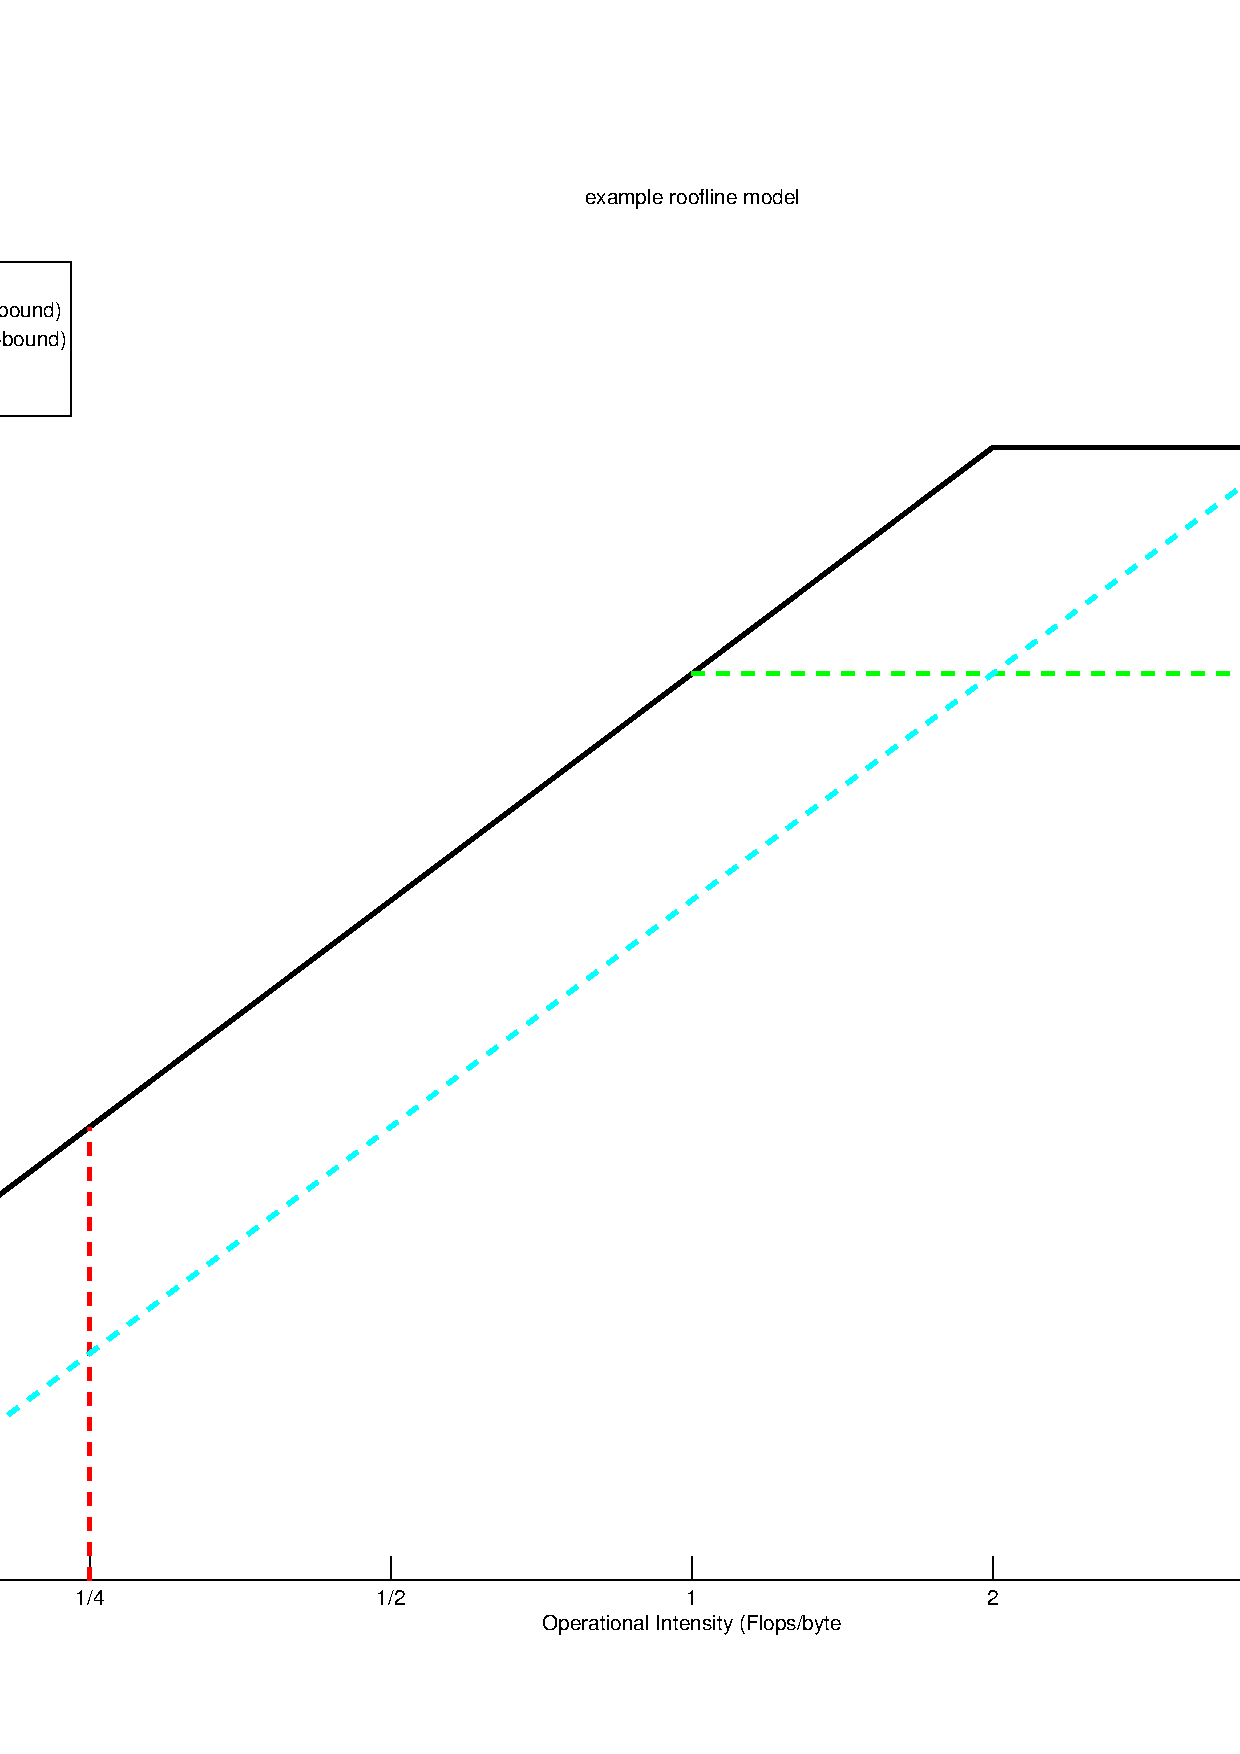
\includegraphics[scale=0.6]{./images/matlab_plots/roofline_example.png}
\caption{Example of a roofline model}
\label{img:roofline_example}
\end{figure}

Although the roofline model has been conceived as a tool for the estimation of performance of multicore CPU architectures, it has been adapted for use with other architectures such as GPU's\cite{spieringsembedded} and FPGA's\cite{spieringsembedded,daperformance}.
The roofline model in it's default form is inadequate to describe the maximum attainable performance of an FPGA based system because of the flexibility of FPGA's. In \cite{daperformance} a number of extensions are proposed to make the roofline model more suitable for FPGA's:
\begin{description}
	
	\item[Operations] Because floating-point operations are prohibitively expensive area-wise, they are often replaced by alternatives such as fixed-point operations. For this reason byte-operations [Bops] are proposed as a more general alternative to the more CPU/GPU specific floating-point operations.

	\item[Scalability] A processing element (PE) is defined as the hardware that contains all the necessary resources to perform the functionality of the algorithm. If the FPGA has enough resources this allows for multiple instantiations of the PE. The scalability factor is given by following formula:

	\begin{equation}
		SC = \left[\frac{Available\;Resources}{Resource\;consumption \; per \; PE}\right]
	\end{equation}

	The attainable performance of one PE needs to be multiplied by the scalability factor.

	\begin{equation}
		Attainable \; Performance = min(CP_{PE} \times SC, CI \times BW)
	\end{equation}

	This relates computational performance to resource consumption.

	\item[I/O bandwidth] In the original roofline model the off-chip memory is considered as the only bound on the performance of a system. Because of the nature of FPGA's where multiple means of I/O are available at the same time these all have to be considered. The roofline model should all take these into consideration and thus have an I/O bandwidth roof and possibly multiple I/O bandwidth ceilings.

	\item[Roofs and ceilings] Due to the fact that the computational intensity and the computational performance are both dependent on the implementation of the algorithm, the computational performance roofline will no longer be a constant. Also a number of ceilings have to be included to represent the different optimization and I/O possibilities.

	\item[Computational intensity] Because the CI influences both the SC and the CP$_{PE}$, it is the key to determining the roofline model. In the original roofline model the CI is modified through the use of code adjustments or optimizations. In the roofline model for FPGA the preferred methods of modifying the CI is through optimizations or through increasing the data locality of the implementation. An example of an optimization that influences the CI is loop unrolling.

\end{description}

\section{Factors influencing performance in a Vivado HLS core}

Video processing systems usually employ buffers to benefit from spatial and temporal locality of reference. In the example of the TRD there are 2 abstractions implemented: \texttt{ap\_linebuffer} and \texttt{ap\_window}.

\subsection{\texttt{ap\_linebuffer} Class}

The class \texttt{ap\_linebuffer} is a generic C++ implementation of the linebuffer described in XAPP793. A linebuffer is described as a multi-dimensional shift-register. A linebuffer needs to be able to be read and written to in the same cycle to maximize performance. The dual port nature of block RAM makes it the ideal component for this abstraction.
Because the \texttt{ap\_linebuffer} class is generic its behavior needs to be defined in the application. The template for the \texttt{ap\_linebuffer} class is \texttt{<typename T, int LROW, int LCOL>}. A type, the number of rows and the number of columns need to be specified. These definitions are in the \texttt{sobel.h} file:


\skipbig{\hlsdirective{typedef ap\_linebuffer<unsigned char, 3, MAX\_WIDTH> Y\_BUFFER;}}


The parameters of the template are used to determine the size of the only variable of the class, -the array M of type T with LROW rows and LCOL columns.\\
This array gets partitioned by the following directive:

\skipbig{\hlsdirective{\#pragma AP ARRAY\_PARTITION variable=M dim=1 complete}}


This means that the first dimension, the number of rows, get partitioned into different block RAMs. This is also reported by the Vivado HLS tool. buff\_A is the line buffer used throughout the implementation.\\

\medskip

\begin{figure}[h]
\centering
\includegraphics[scale=0.8]{/home/frank/School/thesis_text/images/trd_original_buffer_partitioning.PNG} 
\caption{Partitioning of an array in multiple block RAM instances}
\end{figure}


\subsection{\texttt{ap\_window} Class}

The second class used in the application is a generic implementation of the memory window described in XAPP793. It is a combination of shift-registers forming a 2-dimensional data storage element of N pixels centered on a pixel P. Usually these are implemented as flip-flops because they contain relatively few elements who need to be simultaneously available for a calculation. This is achieved through completely partitioning the memory into registers, preventing it from being implemented by a block RAM.
The template of \texttt{ap\_window} is \texttt{<typename T, int LROW, int LCOL>}. These parameters are used for the only variable in the class, an array M of type T with LROW rows and LCOL cols. Analog to the linebuffer class the programmer here also needs to define the type, number of rows and number of columns of array M. The array gets partitioned into registers by the following directive


\skipbig{\hlsdirective{\#pragma AP ARRAY\_PARTITION variable=M dim=0 complete}}


The \texttt{dim=0} means that all dimensions should be partitioned. The \texttt{complete} keyword signifies that this partitioning should be done for the whole array.


\subsection{Influence of memory architecture on the computational intensity}

This hierarchical structure of the memory influences the computational intensity of the algorithm. The numerator is determined by the number of bytes being processed by the core. Every iteration one value gets read from the external memory and one value gets written.  There are 32 bits per pixel, so there are 4 bytes per pixel. This means that with height H and width W there are:

\begin{equation} \label{eq:orig_den}
4 * 2 * ( H * W )
\end{equation}

bytes being read or written to or from the memory. This is the denominator in the expression of the computational intensity.\\
The numerator is dependent on the number of pixels being calculated by the core. The implementation of the Sobel core doesn't calculate the values on the pixels of the outer rim, as can be seen in code listing \ref{lst:sobelpix}

\begin{lstlisting}[caption=Sobel Code Snippet, captionpos=b, label=lst:sobelpix]

if( row <= 1 || col <= 1 || row > (rows-1) || col > (cols-1)){
		
		edge.R = edge.G = edge.B = 0;
		
}
//Sobel operation on the inner portion of the image
else{

		edge = sobel_operator( ... );
		
}

\end{lstlisting}

This however doesn't influence the computational intensity if one interprets a processing element as being all the necessary resources to perform the functionality of the algorithm. Even more so, these pixels also have to be read from memory and are already present in the denominator part of the expression.


\begin{equation} \label{eq:orig_num}
( H * W )
\end{equation}

\medskip
Combining Equations \ref{eq:orig_den} and \ref{eq:orig_num} gives us
\medskip

\begin{equation}
CI = \frac{H \times W}{4 \times 2 \times ( H \times W )}
\end{equation}




\section{Directives influencing throughput}

\subsection{Original Directives}
\label{sec:original_pragma}

The original TRD has 3 directives applied to it:

\begin{itemize}
\item \hlsdirective{set\_directive\_loop\_flatten -off \\ "sobel\_filter/sobel\_filter\_label0"}
\item \hlsdirective{set\_directive\_dependence -variable \&buff\_A -type inter \\ -dependent false "sobel\_filter/sobel\_filter\_label0"}
\item \hlsdirective{set\_directive\_pipeline -II 1 \\ "sobel\_filter/sobel\_filter\_label0"}
\end{itemize}

\paragraph{Throughput}
\label{sec:original_througput}
Given the analysis generated by Vivado HLS, presented in table \ref{tab:analysis_data}, it is possible to calculate the throughput of the system. First of all it needs to be noted whether the system satisfies the timing requirements. The analysis gives us an estimated clock period of 4.2 ns with an uncertainty of 0.62 ns placing it well within the bounds of the required 5 ns clock period.
The system needs 22 cycles to complete. Of these, there are 2 initialization cycles, 20 cycles to finish the outer loop, of which 19 cycles are the inner loop. The system employs pipelining on the innermost loop, which results in an initiation interval of 1.

I denotes a number of iterations, n a number of cycles. N is the number of cycles necessary to calculate one frame:

\begin{equation}\label{eq:nframes_orig_trd}
N_{frame} = n_{init} + I_{outer\;loop} \times ( n_{inner\;loop} + I_{inner\;loop} - 1 )
\end{equation}

% \[
% N =  \text{init cycles} + \text{outer loop iterations} * ( \text{iteration cycles} + \text{inner loop iterations} - 1)
% \]


These cycles all take one clock period to complete:

\begin{equation}\label{eq:frametime}
t_{frame} = N_{frame} * T_{clock}
\end{equation}

The number of frames per second is then given by:

\begin{equation}\label{eq:fps}
FPS = \frac{1}{t_{frame}}
\end{equation}

Entering the numbers found in table \ref{tab:analysis_data} gives us a value of 95.37 frames per second. Given that HDMI has a 60 Hz refresh rate this system satisfies that constraint.


\subsection{No directives}
\label{sec:nopragma}

The original system performance satisfies the real time constraint placed on the system. To study the impact the directives have on the performance of the system, all directives were removed from the  system. The analysis generated by Vivado HLS is presented in the second column of table \ref{tab:analysis_data}. The first observation that can be made is that the system performs the same operation in only 16 clock cycles instead of 22, a decrease of 27\%. Because the system has no pipelining, the initiation interval is 14 cycles. A new value gets read each iteration.

The number of cycles needed to calculate one frame is given by:

\begin{equation}
N = n_{init} + I_{outer\;loop} \times (I_{inner\;loop} \times n_{inner\;loop})
\end{equation}

% \[
% N = init\ cycles + outer\ loop\ iterations * (inner\ loop\ iterations * inner\ loop\ cycles) 
% \]


Knowing the number of cycles the throughput can be calculated using formulas \ref{eq:frametime} and \ref{eq:fps} and the information found in table \ref{tab:analysis_data} . This gives us a value of 0.47 frames per second, a 203 times decrease in performance.

\subsection{Other combinations of directives}

It is clear that these directives have a profound effect on the performance of a system. Also noteworthy is that the directives presented in section \ref{sec:original_pragma} in no way influence the computational intensity of the implementation. Each combination of these directives can thus be represented as a ceiling in the roofline model.
All sensible combinations of these directives have been tested and the results are represented in table  \ref{tab:analysis_data}. The corresponding resource utilization estimates are presented in table \ref{tab:utilization_estimates}.

\paragraph{Only Dependence}
Using only the following directive

\skipbig{\hlsdirective{set\_directive\_dependence -variable \&buff\_A -type inter \\ -dependent false "sobel\_filter/sobel\_filter\_label0"}}

doesn't have any measurable effect on the performance on the system compared to the one presented in section \ref{sec:nopragma}. The calculations for the performance stay the same at 0.47 FPS.

\paragraph{Only Loop Flattening}
Using only the following directive

\skipbig{\hlsdirective{set\_directive\_loop\_flatten "sobel\_filter/sobel\_filter\_label0"}}

combines the 2 loops iterating over the rows and the columns into 1 loop. Because this means that there is only one iteration to take into account, this changes the throughput of the system. The number of cycles necessary to process a frame is given by:

% 1/((init cycles + (outer loop iterations * inner loop iterations) * outer loop cycles)

\begin{equation}
N = n_{init} + (I_{outer\;loop} \times I_{inner\;loop}) \times n_{loop}
\end{equation}

\bigskip

Using formulas \ref{eq:frametime} and \ref{eq:fps} and the values found in \ref{tab:analysis_data}, a performance of 6,88 FPS can be calculated. 

\paragraph{Only pipelining} Using the following directive

\skipbig{\hlsdirective{set\_directive\_pipeline -II 1 "sobel\_filter/sobel\_filter\_label0"}}

Flattens the loops and pipelines them. This has a profound effect on the system performance. II is the initiation interval.

%((Init + outer loop cycles  + ((outer loop iterations * inner loop iterations)-1) * initiation interval)

\begin{equation} \label{eq:only_pipelining}
N  = n_{init} + n_{outer\;loop} + ((I_{inner\;loop} \times I_{outer\;loop}) - 1) \times II
\end{equation}

\bigskip

Using the values found in table \ref{tab:analysis_data} gives a performance of 48.15 FPS. This is a considerable improvement but doesn't reach the required 60 FPS to satisfy the requirements placed on the system by the HDMI protocol. Noteworthy in this case is that the system has an initiation interval of 2. This causes a pixel to be output only every 2 cycles instead of every cycle after the first iteration. The compiler defaults to the lowest II it can use. As an experiment the initiation interval was set to 2 in the directive. This didn't have any measurable influence on the system.

\paragraph{Loop flattening on}
Using following directives:

\begin{itemize}
\item \hlsdirective{set\_directive\_dependence -variable \&buff\_A -type inter \\ -dependent false "sobel\_filter/sobel\_filter\_label0"}
\item \hlsdirective{set\_directive\_pipeline -II 1  \\ "sobel\_filter/sobel\_filter\_label0"}
\item \hlsdirective{set\_directive\_loop\_flatten  \\ "sobel\_filter/sobel\_filter\_label0"}
\end{itemize}

This flattens the loops, pipelines them and takes into consideration that there is no inter-iteration dependence conflict for the buff\_A. The expression for the number of cycles necessary is the same as in equation \ref{eq:only_pipelining}. The most notable difference is that the initiation interval is equal to 1. This gives a performance of 91.72 FPS. Vivado HLS predicts in it's synthesis report that the system will have a minimum clock period 5.25 ns. This leaves the risk that the core will cause glitches and not satisfy the requirements. Increasing the II to 2 makes the system respect the timing constraints again but lowers the performance to 48.15 FPS. 

\paragraph{No dependence}
Using following directives:

\begin{itemize}
\item \hlsdirective{set\_directive\_loop\_flatten -false  \\ "sobel\_filter/sobel\_filter\_label0"}
\item \hlsdirective{set\_directive\_pipeline -II 1  \\ "sobel\_filter/sobel\_filter\_label0"}
\end{itemize}

The only difference with the directives of the original TRD is that the compiler isn't notified of the fact that there is no inter-dependence for the \texttt{buff\_A} variable. The same equation for the performance is given by eq. \ref{eq:nframes_orig_trd}. Using the values found in table \ref{tab:analysis_data} a performance of 95.31 FPS cam be calculated, only marginally worse than the performance of the original configuration. 


\section{Resource consumption}

The resource consumption estimates for these different solutions are given in table \ref{tab:utilization_estimates}. The utilization estimates are of importance because they determine the scalability of a core and thus the maximum attainable performance. Of all the combinations of directives that were tested only the original configuration and the no\_dependence configuration satisfied the requirements for the system. Given that the resource consumption is identical for the original configuration and the no\_dependence configuration the only determining factor in choosing is the performance. Given that the original configuration has better performance, although marginally, it is the most sensible choice to use for the building of a roofline model.\\



% Table specifying the resource consumption of the different solutions

\begin{table}[H]
\begin{center}
\begin{tabular}{rcccc}
\toprule
 & \textbf{BRAM\_18K} & \textbf{DSP48E} & \textbf{FF} & \textbf{LUT}\\ \midrule
\textbf{Original directives} & 3 & 23 & 1487 & 1412 \\ 
\textbf{No pragma} & 5 & 4 & 802 & 1475 \\ 
\textbf{loop\_flatten\_on} & 3 & 23 & 1764 & 1668 \\ 
\textbf{loop\_flatten\_II\_2} & 3 & 23 & 1777 & 1875 \\ 
\textbf{no\_dependence} & 3 & 19 & 1487 & 1412 \\ 
\textbf{no\_pipeline} & 5 & 4 & 802 & 1475 \\ 
\textbf{only dependence} & 5 & 4 & 786 & 1534 \\ 
\textbf{only loop flattening} & 5 & 8 & 1050 & 1783 \\ 
\textbf{only pipelining} & 3 & 23 & 1851 & 1849 \\ \bottomrule
\end{tabular}
\end{center}
\caption{Utilization Estimates}
\label{tab:utilization_estimates}
\end{table}




The original solution was exported as a Xilinx PCore and connected to the TRD system. This system was synthesized to get a more accurate prediction of the resource consumption. The results are detailed in table \ref{tab:scalability}. The difference between the roofline model of the The first noticeable difference when comparing the HLS estimates to the utilization reported from PlanAhead, found on the FILTER\_ENGINE line of the table, is that only the number of reported DSP blocks remains the same. The differences between the other reported values are likely caused by the addition of the AXI wrapper and possible redundancies in the design. The system also uses a number of IP-cores to perform necessary transformations on the data. They do not need to be duplicated to scale the system so these resources can be considered an overhead. Only the filter engine and the associated DMA engine need to be duplicated.\\
The resource consumption in the Zynq differs from the resource consumption for regular FPGA's in that the available interfaces also need to be considered. The Zynq has 4 AXI High Performance ports and these are the constraining factor on the scalability of the TRD core. The filter engine/VDMA combination can be duplicated 3 times. 

% !TEX root = /home/frank/School/thesis_text/thesis.tex


% \begin{table}[H]
% \begin{center}
% \begin{tabular}{rcccc}
% \toprule
%  & \textbf{Register} & \textbf{LUT} & \textbf{BRAM} & \textbf{DSP48} \\ \midrule 
% \textbf{Total n$^{\circ}$ available} & 319200 & 159600 & 140 & 220 \\ 
% \textbf{Total Used} & 27648 & 25804 & 30 & 39 \\ 
% \textbf{FILTER\_ENGINE} & 1965 & 2156 & 2 & 23 \\ 
% \textbf{Overhead} & 25683 & 23648 & 28 & 16 \\ 
% \textbf{Max  available resources} & 293517 & 135952 & 112 & 204 \\ 
% \textbf{Max possible instances} & 149,37 & 63,057 & 56 & 8,87 \\ 
% \textbf{Rounded} & 149 & 63 & 56 & 8 \\ \bottomrule
% \end{tabular}
% \caption{Scalability of the TRD}
% \label{tab:scalability}
% \end{center}
% \end{table}

% \begin{table}[H]
% \begin{center}
% \begin{tabular}{rcccc}
% \toprule
%  & \textbf{Register} & \textbf{LUT} & \textbf{BRAM} & \textbf{DSP48} \\ \midrule 
% \textbf{Total n° available} & 319200 & 159600 & 140 & 220 \\ 
% \textbf{Total Used} & 27648 & 25804 & 30 & 39 \\ 
% \textbf{FILTER\_ENGINE} & 1965 & 2156 & 2 & 23 \\ 
% \textbf{FILTER\_VDMA} & 4176 & 3883 & 6 & 0 \\ 
% \textbf{Overhead} & 21507 & 19765 & 22 & 16 \\ 
% \textbf{Max  available resources} & 297693 & 139835 & 118 & 204 \\ 
% \textbf{Max possible instances} & 48,48 & 23,16 & 14,75 & 8,87 \\ 
% \textbf{Rounded} & 48 & 23 & 14 & 8 \\ \bottomrule
% \end{tabular}
% \caption{Scalability of the TRD}
% \label{tab:scalability}
% \end{center}
% \end{table}

\begin{table}[H]
\begin{center}
\scalebox{0.75}{
\begin{tabular}{rccccc}
\toprule
 									& \textbf{Register} 		& 	\textbf{LUT}		& 	\textbf{BRAM} 		& 	\textbf{DSP48} 		& \textbf{AXI HP} 	\\ \midrule
\textbf{n$^{\circ}$ available} 		& 		319200 				& 		159600 			& 		140 			& 		220 			& 	4 				\\ \medskip
\textbf{System consumption} 		& 		27648 (8.6\%) 		& 		25804 (16.2\%)	& 		30 (21.4\%)		& 		39 (17.7\%) 	& 	2 (50\%) 		\\ 
\textbf{FILTER\_ENGINE} 			& 		1965 (0.6\%)		& 		2156 (1.4\%)	& 		2 (1.4\%)		& 		23 (10.5\%)		& 	0 				\\ \medskip  
\textbf{FILTER\_VDMA} 				& 		4176 (1.3\%)		& 		3883 (2.4\%)	& 		6 (4.3\%)		& 		0 				& 	1 (25\%)		\\ 
\textbf{Overhead} 					& 		21507 (6.7\%)		& 		19765 (12.4\%)	& 		22 (15.7\%)		& 		16 (7.3\%)		& 	1 (25\%)		\\ 
\textbf{Max  available resources} 	& 		297693 (93.3\%)		& 		139835 (87.6\%)	& 		118 (84.3\%)	& 		204 (92.7\%)	& 	3 (75\%)		\\ \midrule
%\textbf{Max possible instances} & 48,48 & 23,16 & 14,75 & 8,87 & 3 \\ 
\textbf{Max Instances} 				& 		48 					& 		23 				& 		14 				& 		8 				& 	3 \\ \bottomrule
\end{tabular}
}
\caption{Scalability of the TRD}
\label{tab:scalability}
\end{center}
\end{table}

\section{Memory Bandwidth}

The memory bandwidth is the decisive factor in determining the performance of a system. In the case of the Zynq however the PS and PL are connected to the AXI interconnect switches. The different AXI interconnect possibilities all influence the maximum attainable memory bandwidth, as well as the DMA controllers utilizing these interconnects. The DDR memory has a bus width of 32 bits and a clock frequency of 1066MHz Providing a maximum bandwidth of 4264 MB/s \cite{anon._zynq-7000_2013}. The filter engine utilizes an AXI HP interconnect port, which in combination with a DMA controller have an estimates throughput of 1200 MB/s. The datasheet for the AXI VDMA controller v5.04a which is used in the system has similar figures, with a typical throughput of 539 MB/s for the MM2S channel and 542 MB/s throughput for the S2MM channel. These can be used in full-duplex which gives a total bandwidth of 1081 MB/s per AXI HP port\cite{axivdma}.
As the scalability has shown the AXI HP interfaces are the constraining factor on the performance of the system. In the case of the TRD only 3 interfaces can be used. This causes the maximum bandwidth to be $3 \times 1081$MB/s or 3243 MB/s. If all 4 interfaces would be used the DDR bandwidth would be the constraining factor. 

\section{Roofline Model}



\newpage
\begin{landscape}

\begin{table}[H]
\begin{center}

	\begin{tabular}{rccccc}
	\toprule
	 & \textbf{Original directives} & \textbf{No pragma} & \textbf{loop\_flatten\_on} & \textbf{loop\_flatten\_II\_2} & \textbf{no\_dependence} \\ \midrule
	
	\textbf{Estimated Clock (ns)} & 4,2 & 4,35 & 5,25 & 4,2 & 4,2 \\ 
	\textbf{Uncertainty (ns)} & 0,62 & 0,62 & 0,62 & 0,62 & 0,62 \\ 
	\textbf{cycle time (ns)} & 5 & 5 & 5,25 & 5 & 5 \\ 
	\textbf{total cycles} & 22 & 16 & 28 & 29 & 23 \\ 
	\textbf{init} & 2 & 2 & 8 & 8 & 2 \\ 
	\textbf{outer loop} & 20 & 14 & 20 & 21 & 21 \\ 
	\textbf{inner loop} & 19 & 13 & N/A & N/A & 20 \\ 
	\textbf{pipelining outer} & no & no & yes & yes & no \\ 
	\textbf{pipelining inner} & yes & no & N/A & N/A & yes \\ 
	\textbf{Initiation Interval} & 1 & 14 & 1 & 2 & 1 \\ \bottomrule
	\end{tabular}

	\bigskip

	\begin{tabular}{rccccc}
	\toprule
	 & \textbf{no\_pipeline} & \textbf{only dependence} & \textbf{only loop flattening} & \textbf{only pipelining} & \textbf{only pipelining II 2} \\ \midrule
	\textbf{Estimated Clock (ns)} & 4,35 & 4,35 & 4,35 & 4,2 & 4,2 \\ 
	\textbf{Uncertainty (ns)} & 0,62 & 0,62 & 0,62 & 0,62 & 0,62 \\ 
	\textbf{cycle time (ns)} & 5 & 5 & 5 & 5 & 5 \\ 
	\textbf{total cycles} & 17 & 16 & 22 & 31 & 31 \\ 
	\textbf{init} & 2 & 2 & 8 & 8 & 8 \\ 
	\textbf{outer loop} & 15 & 14 & 14 & 23 & 23 \\ 
	\textbf{inner loop} & 14 & 13 & N/A & N/A & N/A \\ 
	\textbf{pipelining outer} & no & no & no & yes & yes \\ 
	\textbf{pipelining inner} & no & no & no & no & no \\ 
	\textbf{Initiation Interval} & 15 & 14 & 14 & 2 & 2 \\ \bottomrule
	\end{tabular}


\end{center}
\caption{Analysis Data}
\label{tab:analysis_data}
\end{table}
\end{landscape}

% \begin{landscape}
% \begin{table}[htbp]
% \begin{center}
% \begin{tabular}{|r|r|r|r|r|r|}
% \hline
%  & \textbf{no\_pipeline} & \textbf{only dependence} & \textbf{only loop flattening} & \textbf{only pipelining} & \textbf{only pipelining II 2} \\ \hline
%  &  &  &  &  &  \\ \hline
% \textbf{Estimated Clock (ns)} & 4,35 & 4,35 & 4,35 & 4,2 & 4,2 \\ \hline
% \textbf{Uncertainty (ns)} & 0,62 & 0,62 & 0,62 & 0,62 & 0,62 \\ \hline
% \textbf{cycle time (ns)} & 5 & 5 & 5 & 5 & 5 \\ \hline
% \textbf{total cycles} & 17 & 16 & 22 & 31 & 31 \\ \hline
% \textbf{init} & 2 & 2 & 8 & 8 & 8 \\ \hline
% \textbf{outer loop} & 15 & 14 & 14 & 23 & 23 \\ \hline
% \textbf{inner loop} & 14 & 13 & N/A & N/A & N/A \\ \hline
% \textbf{pipelining outer} & no & no & no & yes & yes \\ \hline
% \textbf{pipelining inner} & no & no & no & no & no \\ \hline
% \textbf{Initiation Interval} & 15 & 14 & 14 & 2 & 2 \\ \hline
% \end{tabular}
% \end{center}
% \caption{Analysis Data Continued}
% \label{tab:analysis_data_cont}
% \end{table}
% \end{landscape}





\emptypage

% !TEX root = /home/frank/School/thesis_text/thesis.tex


\chapter*{Conclusion}

The performance of a heterogeneous processor such as the Zynq is influenced by a number of factors. The first one being the way the memory is implemented. The use of buffers increases the computational intensity, moving the performance of the system further to the right and closer to the peak computational performance. Another factor that plays an important role in the memory architecture is the type and the amount of AXI interconnects that is being used. The AXI HP interconnect has the highest performance for large datasets. The Zynq has 4 on board and only if all 4 are employed at the same time the DDR memory bandwidth becomes the bottleneck. As the TRD shows using the 4 AXI HP ports purely for performing the required action is an unlikely scenario. Using a High Level Synthesis tool presents a serious advantage in programmer productivity. HLS tools such as Vivado HLS give meaningful reports after synthesis and enable a designer to act upon this information. This is in stark contrast to having to synthesize the complete system, which can take up to an hour for a design the size of the TRD.\\
The second factor influencing the performance are the directives applied to the system. As the test shows these can have an immense impact on the performance of a system. Using the solution feature of Vivado the effect of different directives can also be measured in mere minutes. Some of these directives, such as loop unrolling, can influence the computational intensity of the system. Most directives however don't have this effect and can be represented in the roofline models as ceilings for the computational performance.\\
A third factor influencing the performance of the system is the resource consumption. In the case of the TRD a number of IP cores are necessary to transform, read and write the data. Also for every duplicate of the core performing the required action a DMA controller is necessary. Finally due to the low amount of AXI ports these will usually be the constraining factor in scaling the system.\\
The Zynq SoC presents an interesting hybrid between a CPU and an FPGA with serious performance, especially when considered in an embedded system context. Pairing this with a powerful HLS tool allows the designer to get performance from this system relatively quickly.

\emptypage

\bibliographystyle{plain}
\bibliography{Masterproef,old_ref}


\end{document}

   